\chapter{Echtzeitaktualisierung mit WebSockets}
Das wohl spannendste Thema und die erste große Erweiterung dieser Arbeit ist die Echtzeitaktualisierung im Hintergrund der Web-App.

\section{Einführung in WebSockets}
Mit der HTML5-Spezifikation wurden \emph{WebSockets}, ein auf \emph{TCP} basierendes Protokoll der Anwendungsschicht, eingeführt, welches eine Vollduplex, bidirektionale, Single-Socket Verbindung ermöglicht \cite[S. 7]{ws}. Eine Anfrage öffnet die Verbindung zum WebSocket Server (kurz: WS Server) und kann beliebig lange offen gehalten werden, wobei zu jeder Zeit Daten zwischen Client und Server ausgetauscht werden. Dieser Datenaustausch geschieht sehr schnell und mit einem sehr kleinen Overhead, da die Verbindung nicht neu aufgebaut werden muss und die Daten somit sofort verschickt werden können.\\
Ähnlich wie \glqq normale\grqq{} Sockets werden WebSockets von einer Anwendung erzeugt und stellen dann die Schnittstelle zwischen der Webanwendung und dem Transportprotokoll TCP dar.\\
Im direkten Vergleich zu den normalen generischen Sockets, erfüllen WebSockets eine ähnliche Funktion, sind allerdings auf Webanwendungen und TCP beschränkt. 

\paragraph{Handshake} 
Der Handshake erfolgt über HTTP/1.1 und ähnelt dem zum Aufruf einer Homepage.
\\
\begin{lstlisting}[captionpos=b, caption=HTTP Request des Clients {\cite[S. 6]{rfc6455:handshake}}]
  GET / HTTP/1.1
  Host: server.example.com
  Origin: http://www.example.com
  Sec-WebSocket-Key: 7+C600xYyb0v2zmJ69RQsw==
  Sec-WebSocket-Version: 13
  Upgrade: websocket
\end{lstlisting}

Mit \emph{Upgrade: websocket} wird signalisiert, dass der Client eine WebSocket-Verbindung zum Server aufbauen möchte. Der entsprechende WS Server reagiert darauf mit dem HTTP-Statuscode \emph{101 Switching Protocols}, womit er bestätigt, dass er mit dem Wechsel des Protokolls einverstanden ist.
\\
\begin{lstlisting}[captionpos=b, caption=HTTP Response des Servers {\cite[S. 8]{rfc6455:handshake}}]
  101 Switching Protocols
  Connection: Upgrade
  Sec-WebSocket-Accept: fYoqiH14DgI+5y1EMwM2sOLzOi0=
  Upgrade: WebSocket
\end{lstlisting}

Der kryptische Schlüssel \emph{Sec-WebSocket-Accept} muss vom Server berechnet und zurückgegeben werden und zeigt damit, dass er das WebSocket Protokoll versteht. Ab diesem Zeitpunkt ist der Handshake abgeschlossen und die Verbindung wurde aufgebaut.\par

\begin{figure}[!ht]
	\centering
	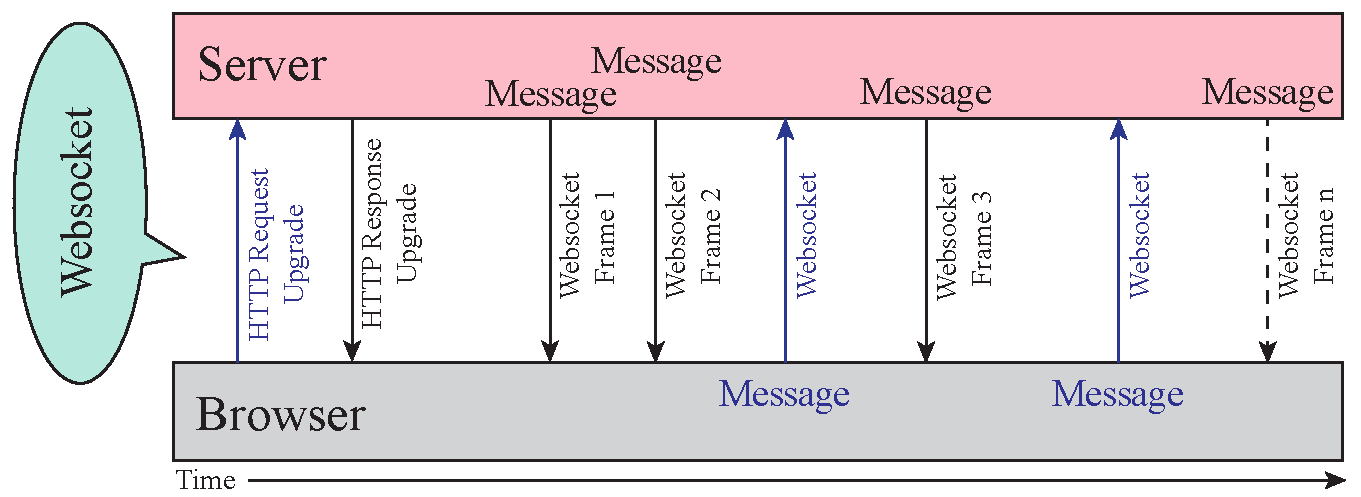
\includegraphics[width=15cm]{fig/websockets}
	\caption[Aufbau einer WebSocket Verbindung]{Aufbau einer WebSocket Verbindung. Danach können beliebig Nachrichten in beide Richtungen (gleichzeitig) übermittelt werden {\cite[S. 7]{ws}}}
\end{figure}

Nun kommen die Vorteile von WebSockets zur Geltung: nach erstmaligem Aufbau der Verbindung bleibt diese geöffnet und zu jedem Zeitpunkt können Client und Server die Vollduplex Verbindung nutzen, um Daten miteinander auszutauschen. So verringern sich die Latenzzeiten, der Traffic und die CPU-Leistung der Server. Das liegt daran, dass die Pakete direkt zugestellt werden können, der Overhead dank einmaligem Handshake deutlich geringer ist und der Austausch der Daten sehr einfach gestaltet ist.

\section{Implementierung der Echtzeitaktualisierung}
Im ersten Ansatz dieser Arbeit wurde der WebSocket-Server auf Basis von \emph{node.js} \cite{node.js}, einem serverseitigem JavaScript Framework für Server, implementiert. Das verlief aufgrund der einfachen Handhabung von WebSockets und der guten Unterstützung von HTML5 problemlos. Jedoch wurden zu diesem Zeitpunkt weder verschlüsselte Verbindungen noch Broadcasting unterstützt. Daher war dies ungeeignet, weil sensible Daten, wie die Standorte der Clients, nicht im Klartext verschickt werden sollten.\\
Außerdem ist eine Broadcast-Funktion notwendig, die den bestehenden Sockets bei Aktualisierung einer Position sofort die neuen Koordinaten übermittelt.\par

Die Implementierung beider Funktionen hätte den Rahmen dieser Arbeit überschritten, weshalb serverseitig das Open Source Modul \emph{socket.io} \cite{socket.io} für node.js verwendet wird. Es stellt sämtliche benötigten Dienste sowie einen Fallback bereit, wodurch auch älteren Browsern ohne HTML5 Unterstützung eine websocketähnliche Verbindung ermöglicht wird.\par

Clientseitig wurde ein Skript in JavaScript entwickelt, welche im Hintergrund der Web-App ausgeführt wird. Es verbindet sich mit dem WebSocket Server, schickt initial die aktuellen Koordinaten unabhängig davon, welcher View gerade angezeigt wird und wartet auf eingehende Nachrichten oder auf eine Änderung der eigenen Position. Bewegt sich der Client, werden automatisch die Koordinaten GoogleMaps-kompatibel in Form von Latitude und Longitude an den WebSocket Server übermittelt.\\
Erhält der Server so eine Nachricht, aktualisiert er seine Datenbank von Standorten der Clients und schickt per Broadcast eine Nachricht an alle verbundenen Clients. So erhalten die Endgeräte in Echtzeit eine Aktualisierung aller Positionen.

\paragraph{Fallback}
Nicht jedes Endgerät unterstützt die Verwendung von WebSockets. Zwar gab es keine Komplikationen mit den getesteten Geräten, da WebSockets mit allen gängigen Desktop Browsern und fast allen mobilen Browsern außer Opera Mini lauffähig ist. Bei veralteter Software ist eine eine Unterstützung jedoch nicht immer gegeben. Daher wurde socket.io so eingerichtet, dass ein Fallback über \emph{flashsockets} hin zum \emph{polling} ermöglicht wird. So kann der größte Teil aller Browser die Echtzeitaktualisierung verwenden.

\paragraph{Entwicklung eines eigenen Protokolls zur Kommunikation über WebSockets}
Um bestimmte Funktionen auf dem Server anzusprechen, wurde ein einfaches Protokoll entwickelt, welches angibt, um welchen Inhalt es sich bei der Nachricht handelt. So haben alle Nachrichten, die zwischen Client und Server ausgetauscht werden, ein bestimmtes Format und ein Feld \emph{type}, welches aktuell folgende Werte annehmen kann:

\begin{itemize}
	\item[] \emph{location:} enthält Latitude und Longitude des Clients
	\item[] \emph{syn:} enthält eine Signatur für die Authentifizierung
	\item[] \emph{subscribe:} abonniert bestimmte Events, dazu später mehr
	\item[] \emph{publish:} signalisiert eine Änderung an der Datenbank
	\item[] \emph{message:} eine neue Chat Nachricht hat den Server erreicht und wird per Broadcast an die Clients verschickt
	\item[] \emph{history:} Anfrage eines Clients nach der aktuellen Historie des Chats
\end{itemize}

Der socket.io Server wertet diese Fälle über ein \emph{Switch-Case-Statement} aus und ruft entsprechende Methoden zur weiteren Verarbeitung auf.

\section{Kommunikation zwischen Apache und WebSocket Server}
Bei dem Webserver Apache und dem WebSocket Server socket.io handelt es sich um zwei Anwendungen, die selbstständig und unabhängig voneinander aktiv sind. Beide verwenden das HTTP Protokoll und müssen mit je einem HTTP Request angesprochen werden. Diese Implementierung sieht vor, dass beide parallel auf einem Server ausgeführt und mit verschiedenen Ports angesprochen werden.\\
Um die Berechtigungen des WebSockets Server möglichst gering zu halten und diesen nur für die Echtzeitaktualisierung zu nutzen, hat socket.io keinerlei Rechte, um auf die Datenbank oder andere Elemente der Webanwendung zugreifen zu können. Dadurch bleibt die Kapselung beider Anwendungen erhalten, aber ein weiterer Schritt zur Authentifizierung eines Benutzers ist erforderlich.

\paragraph{WebSockets über PHP mit ElephantIO}
Damit die Meißner App selbst eine Verbindung zum WebSocket Server aufbauen kann, ist die Open Source Bibliothek \emph{ElephantIO} \cite{elephant.io} erforderlich. Sie ermöglicht die Kommunikation mit Apache und socket.io, da diese sonst nicht (auch nicht über \emph{curl}) ohne Weiteres möglich ist. So gibt es die Funktion, dass die Webanwendung selbst Nachrichten an den WS Server schicken kann.\\
Die Kommunikation in die andere Richtung ist nicht notwendig, da die Web-App keine Informationen benötigt welche Endgeräte sich über WebSockets angemeldet haben.

\section{Authentifizierung eines Clients beim WebSocket Server}
In der Webanwendung auf dem Apache kann mit einem normalen Formular der Benutzername und das Passwort eingegeben werden, allerdings hat der WS Server bekanntlich keinen Zugang zur Datenbank. Es muss aber eine Authentifizierung am WebSocket Server stattfinden, damit nur Benutzer aus der Webanwendung eine Verbindung erstellen können. Dafür wird das \emph{RSA Kryptosystem} verwendet.

\paragraph{Erzeugung der Schlüssel}
Zur ersten Initialisierung der Webanwendung erstellt die Webanwendung sich selbst mittels RSA Verfahren einen privaten $K^-_A$ und einen öffentlichen $K^+_A$ Schlüssel. Sie gehören ausschließlich der Meißner App selbst und werden lokal gespeichert. Der öffentliche Schlüssel wird dem WebSocket Server bereitgestellt, welcher sich diesen direkt aus dem entsprechenden Ordner in der Webanwendung laden kann. Das ist sinnvoll, weil WS Server und Webanwendung sich vertrauen können, da sie auf einer Maschine laufen.

\paragraph{Signieren der Nachricht und anschließende Authentifizierung}
Wenn sich nun ein Client in der Webanwendung mit Benutzernamen und Passwort erfolgreich einloggt, nimmt die App diese Nachricht $m$ und erstellt mit dem privaten Schlüssel eine Signatur $K^-_A(m)$, welche dem Client zur Verfügung gestellt wird. Damit kann dieser nun einen syn-Request mit Benutzernamen, Passwort und Signatur an den WebSocket Server schicken. Der WS Server überprüft nun die Signatur mit dem öffentlichen Schlüssel $K^+_A(K^-_A(m))$ und wenn diese der ursprünglichen Nachricht entspricht, ist der Client authentifiziert.

\begin{figure}[!ht]
	\centering
	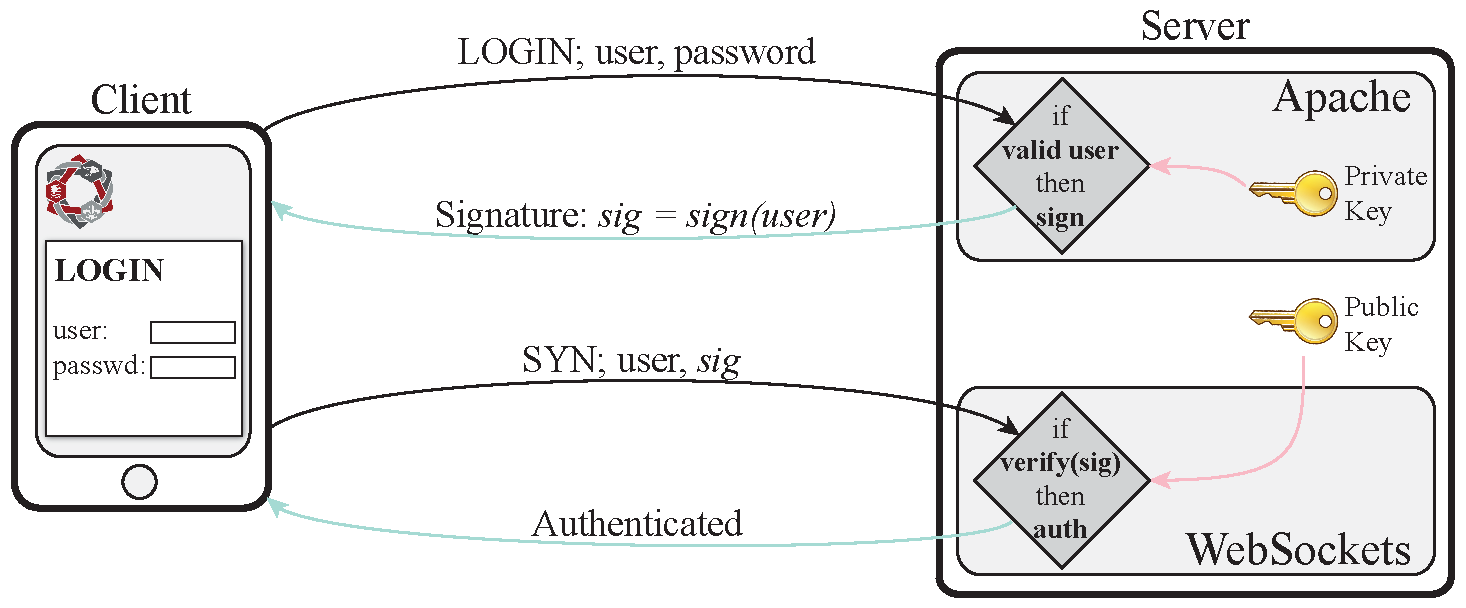
\includegraphics[width=15cm]{fig/publicprivate}
	\caption{Authentifizierung eines Clients beim Server}
\end{figure}

\paragraph{Vorteile dieser Implementierung}
Durch diese Authentifizierung kann socket.io alle eingehenden Verbindungen ablehnen, die keine korrekte Signatur erhalten haben. Ein Angreifer muss somit über den Benutzernamen und das Passwort eines Benutzers verfügen, um sowohl zu der Webanwendung als auch zum WS Server einen Zugang zu erhalten. Er kann nun aber nicht mehr ohne diese Daten eine Verbindung aufbauen und Daten abgreifen.\par

Dieser Weg der Authentifizierung wurde gewählt, da zum Zeitpunkt des Logins der WebSocket des Endgeräts noch nicht bekannt ist. Also kann der Apache dem WS Server nicht mitteilen, welcher Benutzer zu welchem WebSocket gehört. Ein zweiter Schritt zur endgültigen Authentifizierung über eine Signatur ist also notwendig für die korrekte Zuordnung vom offenen WebSocket zum Benutzer. 


\section{Vor HTML5: Benutzung von Polling}
Für den Datenverkehr von Internetseiten wird bekanntlich HTTP benutzt, welches die wechselseitige Datenübermittlung \emph{Halbduplex} verwendet. So erfolgt der Datenverkehr nur in eine Richtung zur gleichen Zeit: der Client schickt eine Anfrage an den Server und dieser übermittelt danach die Antwort \cite[S. 5]{ws}. Das hat wiederum zur Folge, dass es relativ ineffizient ist, da man mit jeder Anfrage stets die Antwort des Servers abwarten muss.\par

\begin{figure}[!ht]
	\centering
	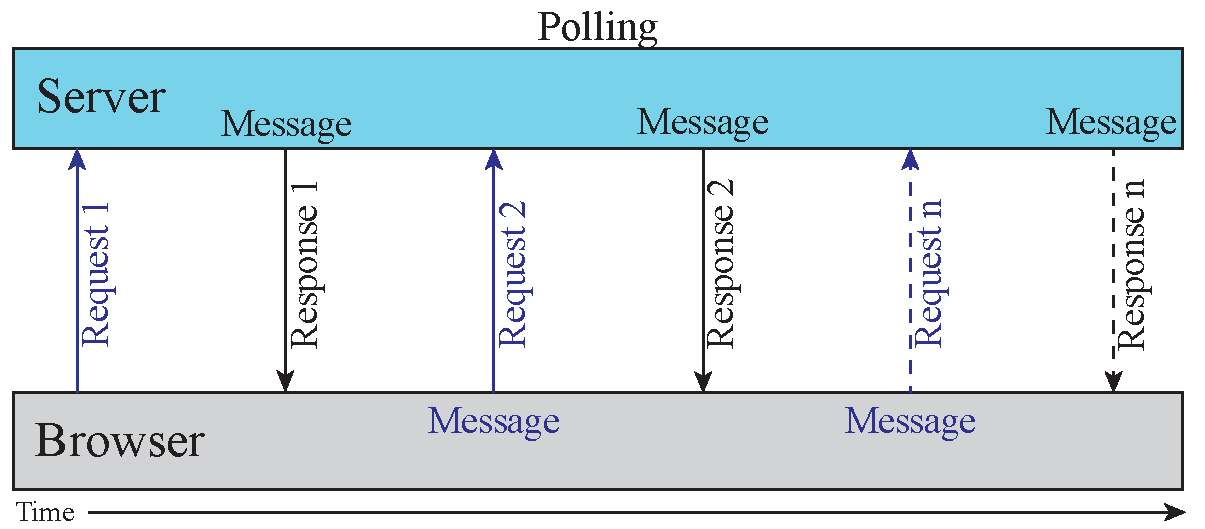
\includegraphics[width=15cm]{fig/polling}
	\caption[Datenaustausch beim Polling]{Datenaustausch mittels HTTP Request / Response beim Polling {\cite[S. 7]{ws}}}
\end{figure}

Vor diesem technischen Hintergrund wurde \emph{Polling} entwickelt, bei dem in einem zeitlich bekannten Intervall eine Anfrage an den Server geschickt wird mit der Bitte um Aktualisierung. Diese Technik ist sehr attraktiv, wenn die zeitlichen Abstände der Aktualisierung der Daten bekannt ist, allerdings sind Echtzeitdaten schlecht vorhersehbar. Dadurch ist Polling nicht die richtige Wahl für dieses Projekt, weil es auf eine wirkliche Echtzeitaktualisierung ankommt.\par

Da bei sämtlichen Techniken, die dem echtzeitähnlichen Austausch von Daten dienen, höhere Latenzen, mehr Rechenleistung und ein komplizierterer Aufbau zu erwarten sind, ist HTML5 mit WebSockets auf dem aktuellen Stand der Dinge und kann vieles besser machen als seine Vorgänger, weshalb für diese Arbeit auch auf diese junge Technik zurückgegriffen wird. Pollingähnliche Verbindungen werden bei dieser Webanwendung nur angewendet, wenn HTML5 oder die WebSockets von dem verwendeten Browser nicht unterstützt werden.